
%%%%%
%%%%% DO NOT EDIT THIS FILE
%%%%%



\documentclass[12pt,a4paper,fleqn]{report}

%%% packages for mathematical typesetting
\usepackage{amsmath}
\usepackage{amssymb}
\usepackage{times}
\usepackage{bm}
%\usepackage{mathtools}
%\usepackage{nicefrac}
%\usepackage{latexsym}

%%% packages for including figures and subfigures
\usepackage{graphicx}
\usepackage[font=footnotesize,labelformat=empty]{subfig}

%%% package for nicer table layout
\usepackage{booktabs}

%%% package for color mangement
\usepackage[svgnames]{xcolor}

%%% package for page headings and footers
\usepackage{fancyhdr}

%%% package for hyperlinks
\usepackage{hyperref}
\hypersetup{%
  colorlinks=true,
  urlcolor=DarkGreen,
  citecolor=green,
  bookmarks=false}


\usepackage[noend]{algpseudocode}
\algrenewcommand\algorithmicdo{}
\algrenewcommand\algorithmicthen{}
\algrenewcommand{\algorithmiccomment}[1]{// #1}
\makeatletter
\newcommand{\StatexIndent}[1][3]{%
  \setlength\@tempdima{\algorithmicindent}%
  \Statex\hskip\dimexpr#1\@tempdima\relax}
\makeatother


\usepackage{fancyvrb} 
\usepackage{listings}
% Python style / environment for highlighting in "figures"
\lstdefinestyle{pythonstyle}{%
  language=Python,
  tabsize=4,
  backgroundcolor=\color{Gray!10},
  basicstyle=\ttfamily\scriptsize,
  stringstyle=\color{ForestGreen},
  keywordstyle=\color{BlueViolet},
  commentstyle=\itshape\color{DarkRed!90},
  identifierstyle=,
  emphstyle=\color{Blue},
  frame=lines,	
  showstringspaces=false,
  morekeywords={range, len, self, lambda, from, import, as, False, True, enumerate, map, list, set, float, int, min, max, with}
  fancyvrb=true,
}
\lstnewenvironment{python}[1][]{\lstset{style=pythonstyle,#1}}{}





\graphicspath{{./Figures/}, {./Images/}}



%%% text highlighting
\newcommand{\keyword}[1]{\emph{\texttt{\color{blue}#1}}}
\newcommand{\alert}[1]{\emph{\texttt{\color{red}#1}}}


%%% sets
\newcommand{\set}[1]{#1}

%%% vectors, matrices, and tensors
\renewcommand{\vec}[1]{\bm{#1}}
\newcommand{\mat}[1]{\bm{#1}}
\newcommand{\ten}[1]{\bm{\mathcal{#1}}}

%%% trace, rank, and diagonal
\newcommand{\tr}[1]{\operatorname{tr} \bigl [ #1 \bigr ]}
\newcommand{\TR}[1]{\operatorname{tr} \Bigl [ #1 \Bigr ]}
\newcommand{\rk}[1]{\operatorname{rk} \bigl [ #1 \bigr ]}
\newcommand{\RK}[1]{\operatorname{rk} \Bigl [ #1 \Bigr ]}
\newcommand{\diag}[1]{\operatorname{diag} \bigl [ #1 \bigr ]}
\newcommand{\DIAG}[1]{\operatorname{diag} \Bigl [ #1 \Bigr ]}

%%% inverse and transpose
\newcommand{\inv}[1]{#1^{-1}}
\newcommand{\trn}[1]{#1^\intercal}
\newcommand{\invtrn}[1]{#1^{-\intercal}}

%%% outer product
\newcommand{\opt}[2]{#1 \trn{#2}}

%%% inner products
\newcommand{\ipt}[2]{\trn{#1} #2}
\newcommand{\iptb}[2]{\left( \ipt{#1}{#2} \right)}
\newcommand{\ip}[2]{\langle #1, #2 \rangle}
\newcommand{\Ip}[2]{\bigl \langle #1, #2 \bigr \rangle}
\newcommand{\ipa}[2]{\langle #1, #2 \rangle}
\newcommand{\Ipa}[2]{\bigl \langle #1, #2 \bigr \rangle}
\newcommand{\dsq}[2]{\bigl \lVert #1 - #2 \bigr \rVert^2}
\newcommand{\nrm}[1]{\bigl \lVert #1 \bigr \rVert^2}
\newcommand{\sdsq}[2]{\lVert #1 - #2 \rVert^2}
\newcommand{\snrm}[1]{\lVert #1 \rVert^2}


\newcommand{\st}{\operatorname{s.\!t.}}
\newcommand{\amin}[1]{\operatorname*{argmin}_{#1}}
\newcommand{\amax}[1]{\operatorname*{argmax}_{#1}}

\newcommand{\submax}[1]{#1_{\text{max}}}

\newcommand{\ci}{\perp\!\!\!\perp}
\newcommand{\prob}[1]{p\bigl( #1 \bigr)}
\newcommand{\cprob}[2]{p\bigl( #1 \bigm| #2 \bigr)}

%%% horizontal and vertical dash
\newcommand{\hdash}{\operatorname{\,{}---{}\,}}
\renewcommand{\vdash}{\arrowvert}





\pagestyle{fancy}
\lhead{\emph{Image Processing (1)}}
\rhead{\emph{Winter Term 2021/22}}
\cfoot{}

\frenchspacing

\setlength{\parskip}{1ex plus0.5ex minus0.5ex}

\setlength{\headheight}{15pt}

\def\thesection{\arabic{section}.}
\setlength{\parindent}{0pt}

\renewcommand{\familydefault}{\sfdefault}





\begin{document}

\subsection*{exercise 2}
\textbf{superpixels and tiling effects}
\vspace{1cm}

\subsection*{solutions due}
until \textbf{November 14, 2021} at \textbf{23:59} via \textbf{ecampus}
\vspace{1cm}

\vfill


\subsection*{students handing in this solution set}

\begin{tabular*}{\textwidth}{l@{\extracolsep{\fill}}lll}
  \toprule
  last name & first name & student ID & enrolled with \\
  \midrule
  \midrule
  %%%
  %%% enter data of 1st student here (i.e replace the following place holders)
  %%%
  Bach
  & Franziska
  & 123456
  & B-IT / RWTH Aachen
  \\
  %%%
  %%% enter data of 2nd student here (i.e replace the following place holders)
  %%%
  Wolfe
  & Frank
  & 654321
  & Uni Bonn
  \\
  %%%
  %%% if necessary, i.e. if there are further students in your team, add rows to this table
  %%%
  \bottomrule
\end{tabular*}
\newpage










%%%%%
%%%%% DO NOT EDIT THE FOLLOWING
%%%%%

\subsection*{general remarks}

As you know, your instructor is an avid  proponent of open science and education. Therefore, \textbf{MATLAB implementations will not be accepted} in this course.

The goal of this exercise is to get used to practical image processing in python / numpy / scipy. There are numerous Web resources related to python programming; numpy and scipy are mostly well documented and matplotlib, too, comes with numerous tutorials. Play with the code that is provided. The tasks below are rather simple; if you do not have any ideas for how to solve them, just look around for ideas as to how it can be done.

Also, \textbf{do NOT use additional third party libraries such as \texttt{OpenCV} or \texttt{scikit-image} for the coding tasks in this course!}

Why not? Because our goal in this course and its exercises is to learn about theory and practice of image processing on a reasonably foundational level. Regarding practical implementations of image processing algorithms, solutions in C or even assembler would constitute the most foundational level but likely be unreasonable. While working with python / numpy / scipy is still foundational enough, working with libraries such as \texttt{OpenCV} or \texttt{scikit-image} is definitely not. 

Think of it like this: if you train yourself to become a library monkey then what are you going to do when you are supposed to solve a problem for which there is no convenient library function available? How can you be sure that you really learned how to turn mathematics into computer code if all you ever do is stitching together other people's solutions to seemingly related problems?

\textbf{When handing solutions, always strive for excellence!} Your code and results will be checked and need to be convincing, reproducible, and comprehensible. If your solutions meet these criteria and you can demonstrate that they work in practice, it is a \emph{satisfactory} solution.

A \emph{very good} solution requires additional efforts especially w.r.t. to readability of your code. If your code is neither commented nor well structured, your solution is not good! The same holds for your discussion of your results: these should be concise and convincing and demonstrate that you understood what the respective task  was all about. Striving for very good solutions should always be your goal!
 


\newpage

\subsection*{practical advice}



The problem specifications you'll find below assume that you work with python / numpy / scipy. They also assume that you have imported 
\begin{python}
import imageio
import numpy as np
import scipy.ndimage as img
\end{python}



\vfill
To read- and write images from- and to disc, you may use these functions
\begin{python}[emph={imageRead,imageWrite}]
def imageRead(imgname, pilmode='L', arrtype=np.float):
    """
    read an image file into a numpy array

    imgname: str
        name of image file to be read 
    pilmode: str
        for luminance / intesity images use 'L'
        for RGB color images use 'RGB'
    arrtype: numpy dtype
        use np.float, np.uint8, ...
    """
    return imageio.imread(imgname, pilmode=pilmode).astype(arrtype)


def imageWrite(arrF, imgname, arrtype=np.uint8):
    """
    write a numpy array as an image file
    the file type is inferred from the suffix of parameter imgname, e.g. '.png'

    arrF: array_like
        array to be written
    imgname: str
        name of image file to be written
    arrtype: numpy dtype
        use np.uint8, ...
    """
    imageio.imwrite(imgname, arrF.astype(arrtype))
\end{python}



\vfill
To display an intensity image on your screen, you could use the following
\begin{python}
import matplotlib.pyplot as plt

arrF = imageRead('portrait.png')
plt.imshow(arrF / 255, cmap='gray')
plt.show()
\end{python}



To display an (RGB) color image on screen, you might use
\begin{python}
import matplotlib.pyplot as plt

arrF = imageRead('../exercise1/Data/asterixRGB.png', pilmode='RGB')
plt.imshow(arrF / 255)
plt.show()
\end{python}




\subsection*{task 2.1 \\[1ex] (na\"ive) downsampling}

A rather simple idea for how to reduce the resolution of a digital (intensity) image is to keep only every $m$-th row and every $n$-th column of its pixels. For example, the figure below shows the effect of \emph{downsampling} by a factor of $2$, i.e. \emph{downsampling} by means of choosing $m = n = 2$.

Without using \keyword{for} loops, implement a function \keyword{downsample} with three parameters \texttt{arrF}, \texttt{m}, and \texttt{n} that realizes this manner of downsampling.

For $(m,n) \in \bigl\{ (4,4), (8,8) \bigr\}$, apply your method to image \texttt{portrait.png} and enter your results here
%%%%%
%%%%%
%%%%% enter your result here, i.e. replace "placeholder.pdf" by the names of your resulting image files
%%%%%
%%%%%
\begin{figure}[h!]
\subfloat[$256 \times 256$]{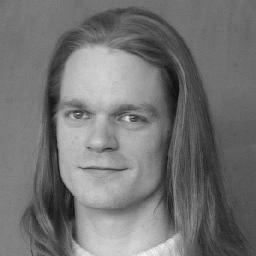
\includegraphics[width=0.40\textwidth]{portrait.png}} \hfill
\subfloat[$128 \times 128$]{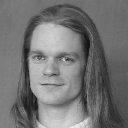
\includegraphics[width=0.20\textwidth]{t2-1-128x128.png}} \hfill
\subfloat[$64 \times 64$]{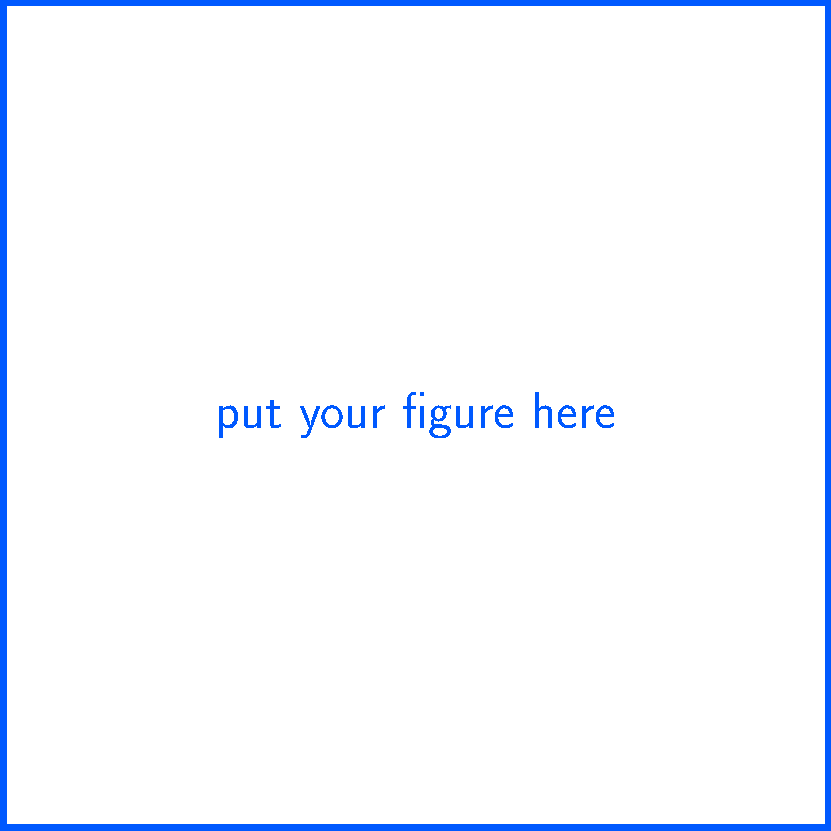
\includegraphics[width=0.10\textwidth]{placeholder.pdf}} \hfill
\subfloat[$32 \times 32$]{\makebox[1.5\width][c]{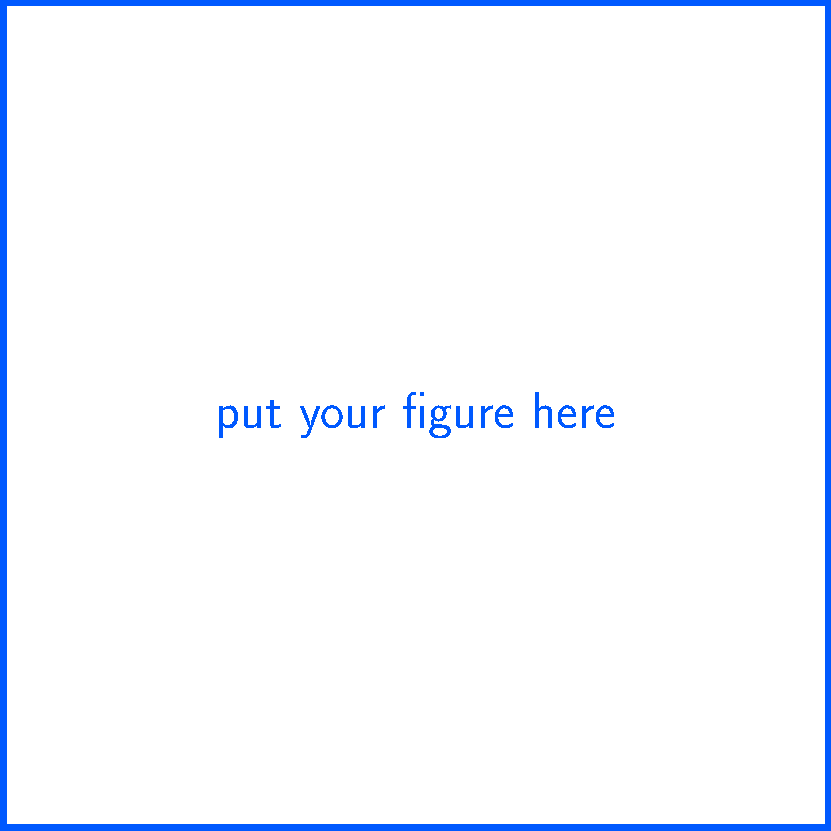
\includegraphics[width=0.05\textwidth]{placeholder.pdf}}}
\end{figure}
%%%%%
%%%%%
%%%%%
%%%%%
%%%%%



\vspace{2cm}
Also, paste your code here 
%%%%%
%%%%%
%%%%% enter your code into the following environment
%%%%%
%%%%%
\begin{python}
# paste your code here

\end{python}
%%%%%
%%%%%
%%%%%
%%%%%
%%%%%


\subsection*{task 2.2 \\[1ex] Kronecker products for (na\"ive) upsampling}

The Kronecker product of an ordered pair of matrices (or 2D \emph{numpy} arrays) $\mat{A}, \mat{B}$ of sizes $k \times l $ and $m \times n$ respectively is defined as
\begin{equation*}
\mat{C} = \mat{A} \otimes \mat{B}
=
\begin{bmatrix}
a_{11} \mat{B} & a_{12} \mat{B} & \cdots & a_{1l} \mat{B} \\
a_{21} \mat{B} & a_{22} \mat{B} & \cdots & a_{2l} \mat{B} \\
\vdots & \vdots & \ddots & \vdots \\
a_{k1} \mat{B} & a_{k2} \mat{B} & \cdots & a_{kl} \mat{B} \\
\end{bmatrix}
\end{equation*}
and therefore produces a matrix (or 2D array) $\mat{C}$ of size $k \cdot m \times l \cdot n$.

Conveniently, \emph{numpy} provides the function \keyword{np.kron()} for the computation of Kronecker products. This allows us to realize a rather simple idea for \emph{upsampling} a small (intensity) image: assuming that the given image is stored in an array $\mat{F}$, we may simply compute
\begin{equation*}
\mat{G} = \mat{F} \otimes \mat{O}
\end{equation*}
where $\mat{O}$ denotes an $m \times n$ array of all ones.

Now, without using \keyword{for} loops, implement an appropriately parameterized function \keyword{upsample}. Then, load image \texttt{portrait.png} into \texttt{arrF} and compute
\begin{python}[emph={downsample,upsample}]
arrG = upsample(downsample(arrF, m, n), m, n)
\end{python}



\vspace{1cm}
Choose $(m,n) \in \bigl\{ (2,2), (4,4) \bigr\}$ and enter your results here (the figure already shows how your result should look like for $m=n=8$) 
%%%%%
%%%%%
%%%%% enter your result here, i.e. replace "placeholder.pdf" by the names of your resulting image files
%%%%%
%%%%%
\begin{figure}[h!]
\subfloat[$m = n = 1$]{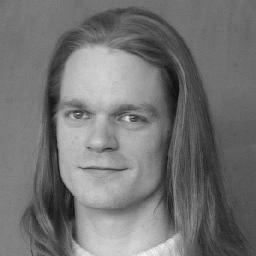
\includegraphics[width=0.24\textwidth]{portrait.png}} \hfill
\subfloat[$m = n = 2$]{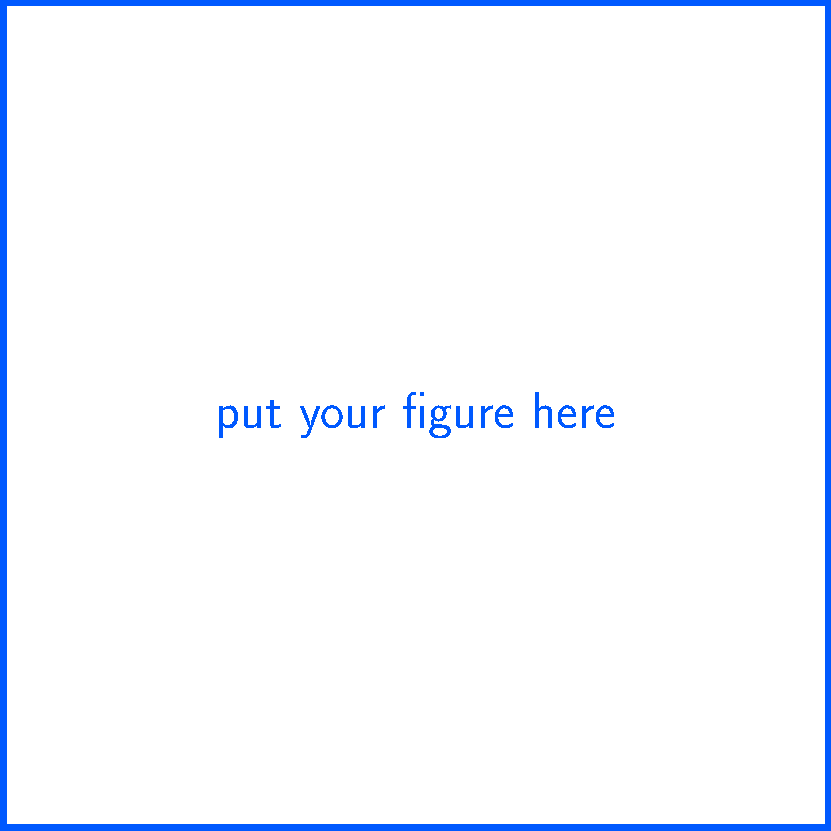
\includegraphics[width=0.24\textwidth]{placeholder.pdf}} \hfill
\subfloat[$m = n = 4$]{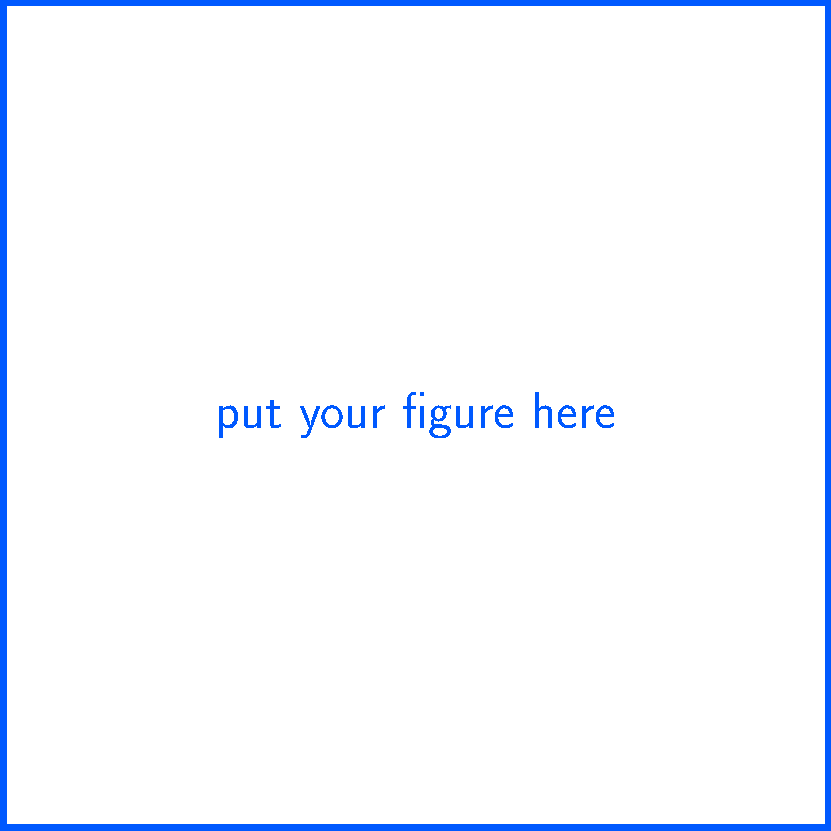
\includegraphics[width=0.24\textwidth]{placeholder.pdf}} \hfill
\subfloat[$m = n = 8$]{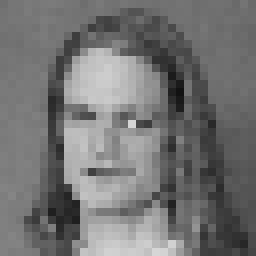
\includegraphics[width=0.24\textwidth]{t2-2-8x8.png}}
\end{figure}
%%%%%
%%%%%
%%%%%
%%%%%
%%%%%








\subsection*{task 2.3 \\[1ex] superpixels (part 1)}

In the previous task, we have already seen examples of images composed of \emph{superpixels}. These are images of size $M \times N$ whose content consists of uniformly colored tiles of size $m \times n$ where $m \ll M$ and $n \ll N$.

In the previous task, the superpixels resulted from (na\"ively) upsampling a small image into a larger one. However, superpixels also arise in an image effect called \emph{pixelize} (which is often used to render faces unrecognizable). In this effect, each pixel in each $m \times n$ tile of a given image is set to the average intensity value within the tile.

\begin{figure}[h!]
\subfloat[given image]{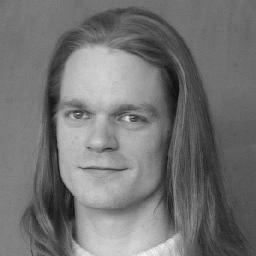
\includegraphics[width=0.32\textwidth]{portrait.png}} \hfill
\subfloat[$8 \times 8$ pixelize]{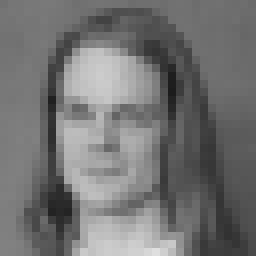
\includegraphics[width=0.32\textwidth]{t2-3-8x8.png}} \hfill
\subfloat[$16 \times 16$ pixelize]{
\includegraphics[width=0.32\textwidth]{t2-3-16x16.png}} 
\end{figure}

\vfill
As always, there are many ways for how to implement this effect. Here is an intuitive C-style implementation that involves four nested \keyword{for} loops
\begin{python}[emph={meanSuperPixelV1,meanSuperPixelV2,meanSuperPixelV3,meanSuperPixelV4}]
def meanSuperPixelV1(arrF, m, n):
    M, N = arrF.shape
    
    arrG = np.zeros((M, N))

    for i in range(0, M, m):
        for j in range(0, N, n):
            intensity_sum = 0
            for k in range(m):
                for l in range(n):
                    intensity_sum += arrF[i+k,j+l]
            intensity_avg = intensity_sum / (m*n)
            arrG[i:i+m,j:j+n] = intensity_avg

    return arrG
\end{python}

\newpage
We don have to be quite so na\"ive but can replace the two innermost \keyword{for} loops using the \emph{numpy} function \keyword{np.mean()}
\begin{python}[emph={meanSuperPixelV1,meanSuperPixelV2,meanSuperPixelV3,meanSuperPixelV4}]
def meanSuperPixelV2(arrF, m, n):
    M, N = arrF.shape
    
    arrG = np.zeros((M, N))

    for i in range(0, M, m):
        for j in range(0, N, n):
            arrG[i:i+m,j:j+n] = np.mean(arrF[i:i+m,j:j+n])

    return arrG
\end{python}

As almost always, \emph{numpy} allows us to get rid of \keyword{for} loops alltogether. Here is a solution inspired by the kind of (unfortunately often stupid) answers you will get when asking the \href{https://stackoverflow.com/questions/14229029/block-mean-of-numpy-2d-array}{\textbf{stackoverflow}} community (we will not even bother discussing this messy mumble \ldots)

\begin{python}[emph={meanSuperPixelV1,meanSuperPixelV2,meanSuperPixelV3,meanSuperPixelV4}]
def meanSuperPixelV3(arrF, m, n):
    M, N = arrF.shape

    arrG = np.reshape(arrF, (M*N//n, n))
    arrG = np.mean(arrG, axis=1)
    arrG = np.reshape(arrG, (M,N//n))

    arrH = np.reshape(arrG, (m, (M//m)*(N//n)), 'F')
    arrH = np.mean(arrH, axis=0)
    arrH = np.reshape(arrH, (M//m, N//n), 'F')

    return np.kron(arrH, np.ones((m,n)))
\end{python}    

Finally, here is how \emph{numpy} black belts implement the pixelize effect (we will discuss this coding pattern later in the course)
\begin{python}[emph={meanSuperPixelV1,meanSuperPixelV2,meanSuperPixelV3,meanSuperPixelV4}]   
def meanSuperPixelV4(arrF, m, n):
    M, N = arrF.shape

    arrA = np.add.reduceat(arrF, np.arange(0,N,n), axis=1) / n
    arrB = np.add.reduceat(arrA, np.arange(0,M,m), axis=0) / m
    arrC = np.repeat(arrB, n, axis=1)
    arrD = np.repeat(arrC, m, axis=0)
    
    return arrD
\end{python}

\textbf{Here is your task:} letting $m=n=8$,  perform runtime measurements for the above four methods on \texttt{portrait.png} and enter your results here
\color{blue} \\[1ex]
%%%%%
%%%%%
%%%%% enter your result here
%%%%%
%%%%%
enter your result here \ldots
%%%%%
%%%%%
%%%%%
%%%%%
%%%%%
\color{black}






\subsection*{task 2.4 \\[1ex] superpixels (part 2)}

Instead of working with the \emph{mean} intensity value in each $m \times n$ tile of an image, we can also pixelize by using \emph{median} intensities.

Implement a function \keyword{medianSuperPixel} simply by replacing \keyword{np.mean()} in \keyword{meanSuperPixelV2} with \keyword{np.median()}.

For $(m, n) \in \bigl\{ (4,4), (32,32), (16,32), (32,16) \bigr\}$, run \keyword{meanSuperPixelV2} and \keyword{medianSuperPixel} on \texttt{portrait.png} and paste your results here \\[1cm]
%%%%%
%%%%%
%%%%% enter your result here, i.e. replace "placeholder.pdf" by the names of your resulting image files
%%%%%
%%%%%
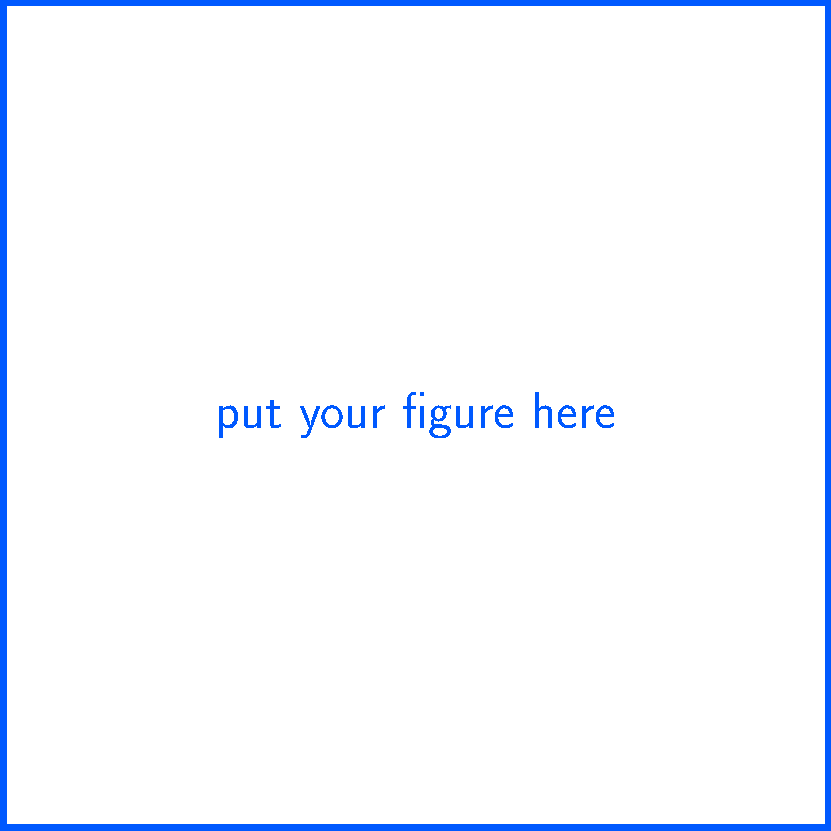
\includegraphics[width=0.24\textwidth]{placeholder.pdf} \hfill
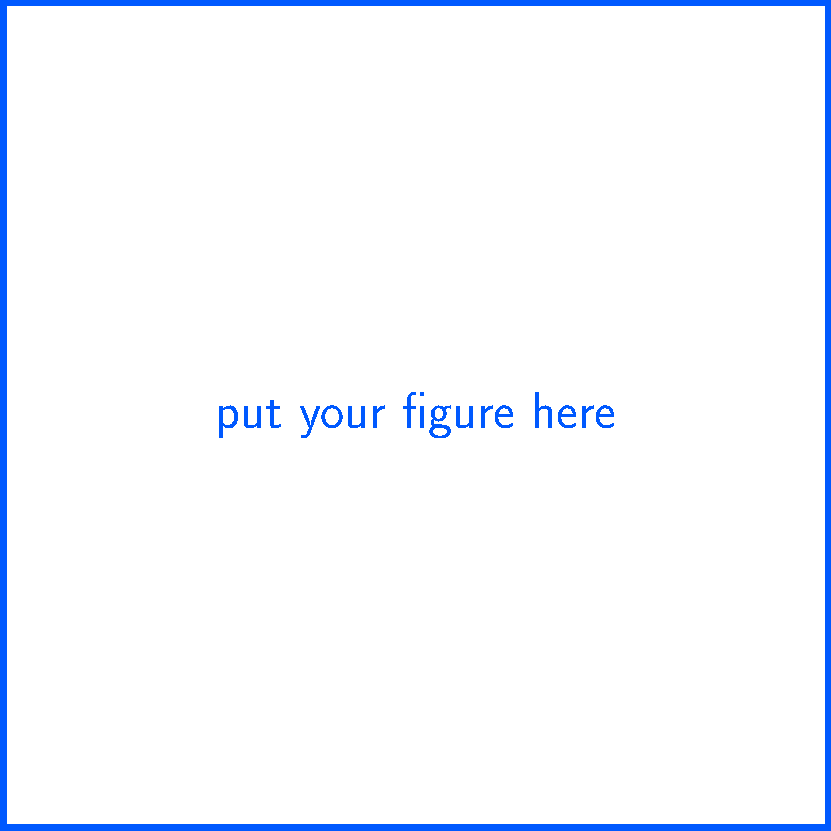
\includegraphics[width=0.24\textwidth]{placeholder.pdf} \hfill
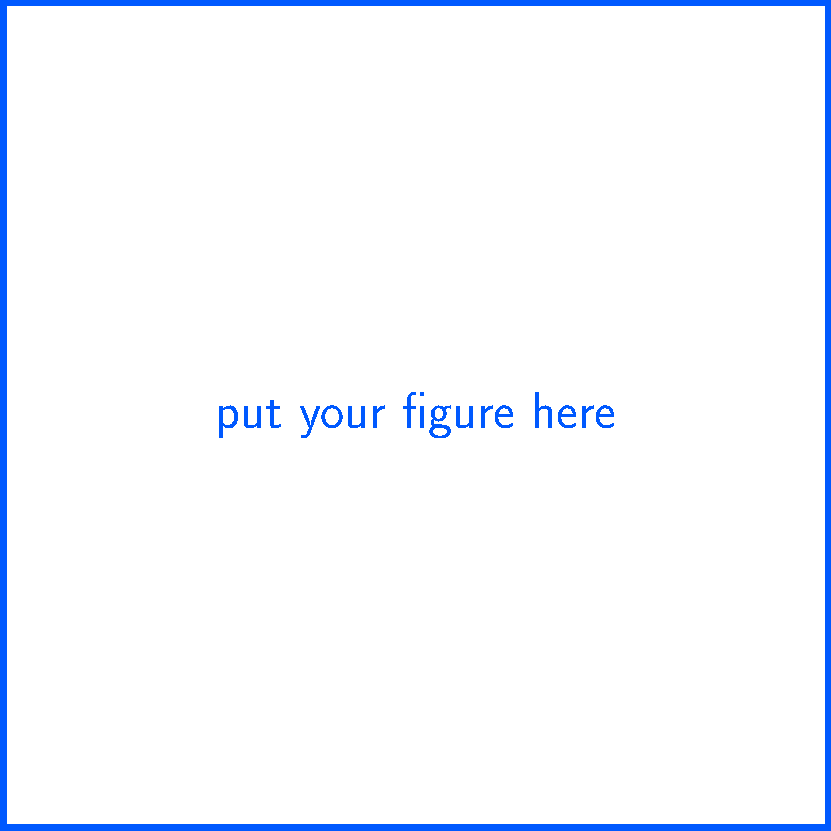
\includegraphics[width=0.24\textwidth]{placeholder.pdf} \hfill
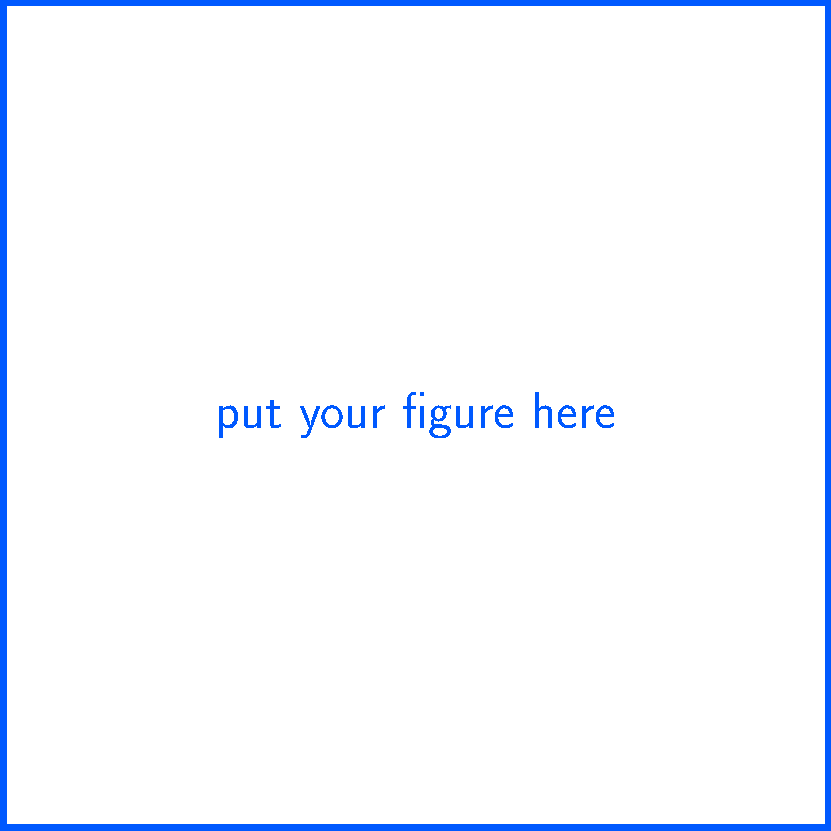
\includegraphics[width=0.24\textwidth]{placeholder.pdf} 

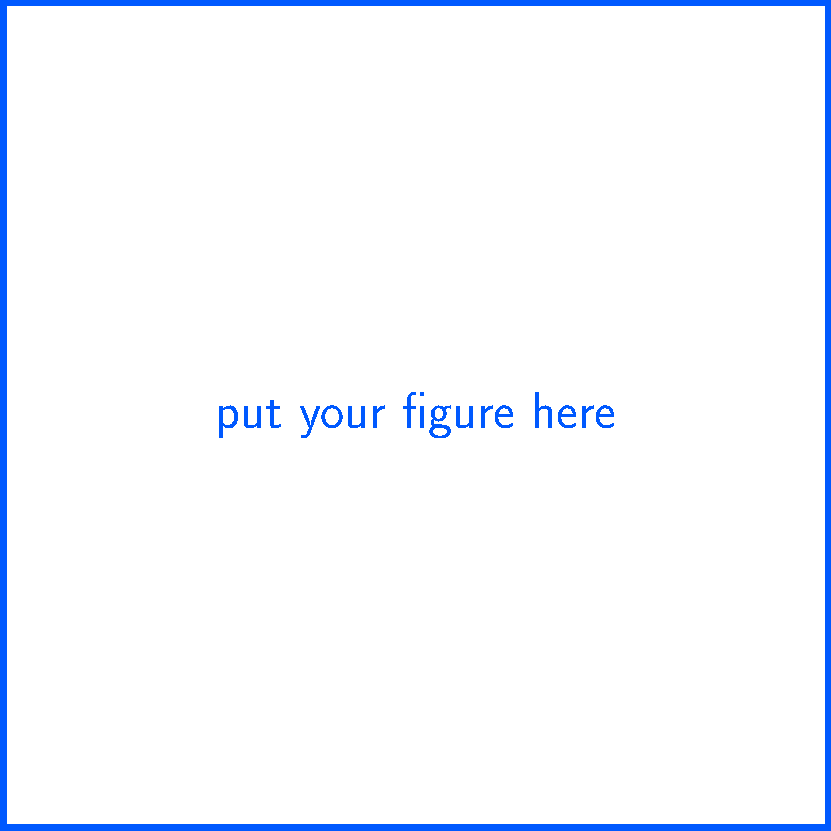
\includegraphics[width=0.24\textwidth]{placeholder.pdf} \hfill
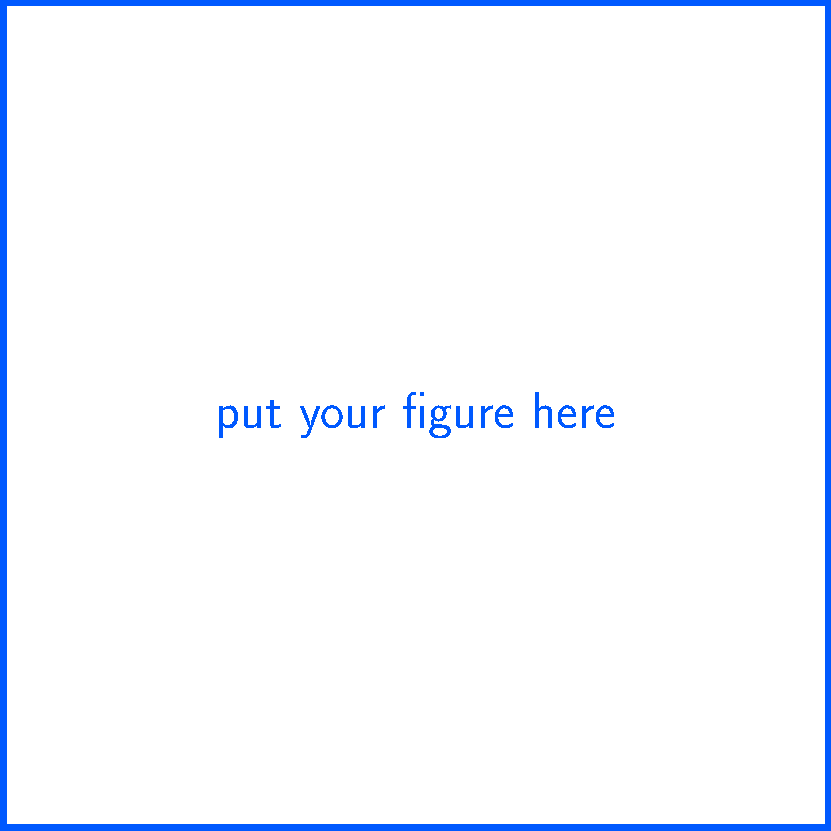
\includegraphics[width=0.24\textwidth]{placeholder.pdf} \hfill
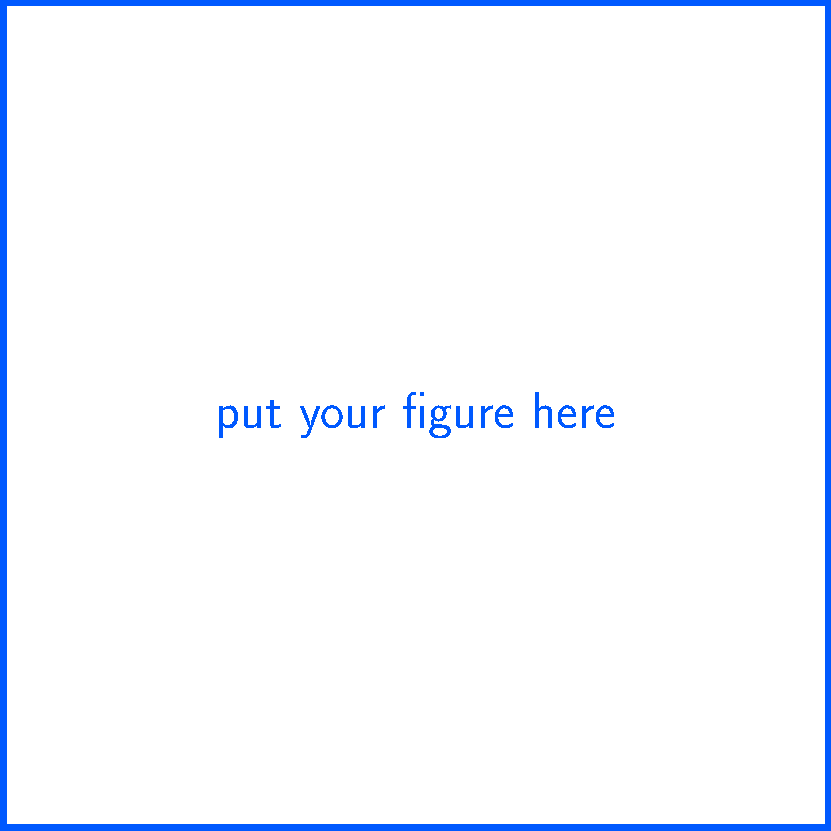
\includegraphics[width=0.24\textwidth]{placeholder.pdf} \hfill
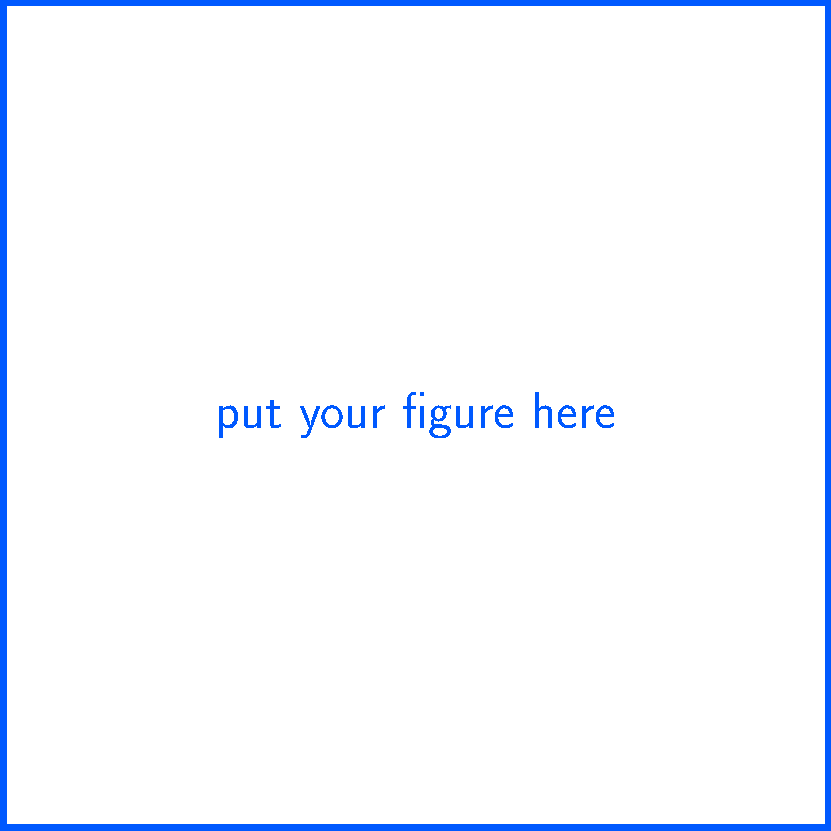
\includegraphics[width=0.24\textwidth]{placeholder.pdf} 
%%%%%
%%%%%
%%%%%
%%%%%
%%%%%







\subsection*{task 2.5 \\[1ex] why do we always work with small images ?}

Some of you may wonder why the example images we consider in these exercises are always rather small (say of resultion $256 \times 256$ pixels) \ldots To make a long story short, this is in order not to tax you patience. We already saw that large images take longer to process. Just for the fun it, let us therefore test your patience and pixelize a larger color image.  

In the \texttt{Data} folder for this exercise, you will find the image
\begin{quote}
    \texttt{bauckhage.jpg}
\end{quote}
This image has a resolution of $4068 \times 2712$ pixels and is therefore still of moderate size given present day standards. Read this color image into a \emph{numpy} array \texttt{arrF}, run \keyword{medianSuperPixel} on each of its color layers, and write your result as a PNG image. Experiment with different tile sizes $m \times n$ and paste one of your results here \\[1cm]
%%%%%
%%%%%
%%%%% enter your result here, i.e. replace "placeholder.pdf" by the name of your resulting image file
%%%%%
%%%%%
\begin{center}
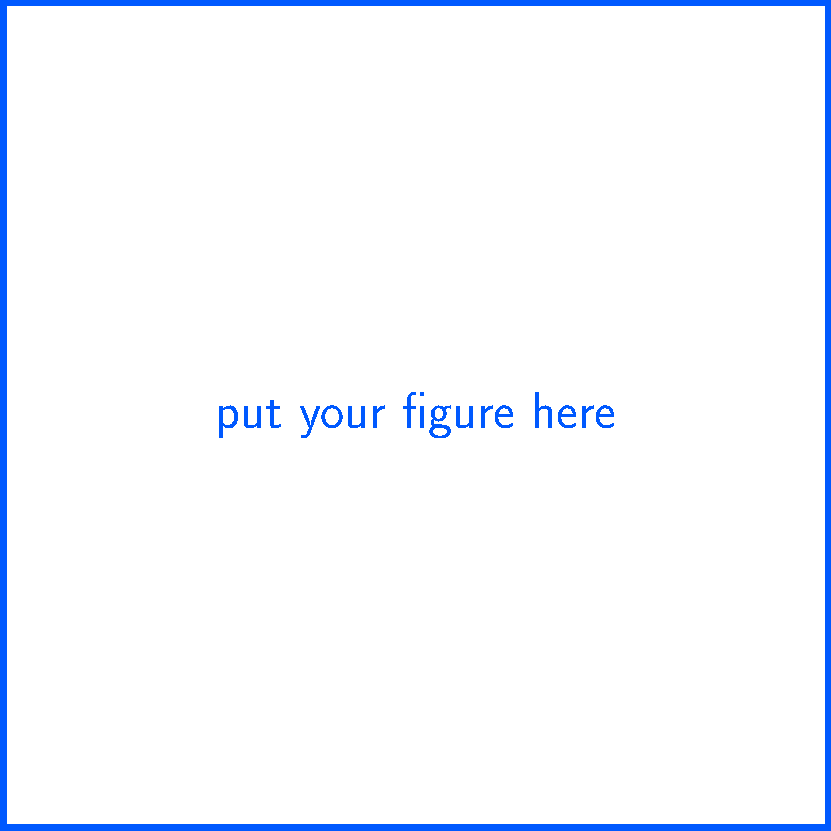
\includegraphics[height=0.4\textwidth,width=0.6\textwidth]{placeholder.pdf} 
\end{center}
%%%%%
%%%%%
%%%%%
%%%%%
%%%%%







\subsection*{task 2.6 \\[1ex] ``simple'' tiling effects}

Speaking of tiles of size $m \times n$, can you think of a piece of code that creates images like these where tiles have been moved around randomly? 
\begin{figure}[h!]
\subfloat[input image]{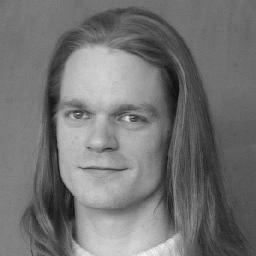
\includegraphics[width=0.24\textwidth]{portrait.png}} \hfill
\subfloat[tile size $8 \times 8$]{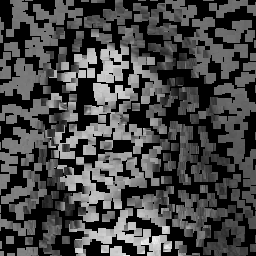
\includegraphics[width=0.24\textwidth]{t2-6-8x8.png}} \hfill
\subfloat[tile size $32 \times 32$]{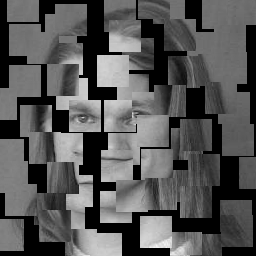
\includegraphics[width=0.24\textwidth]{t2-6-32x32.png}} \hfill
\subfloat[tile size $13 \times 7$]{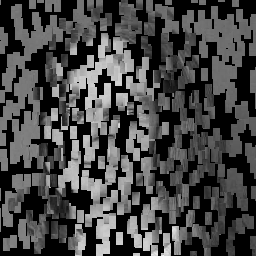
\includegraphics[width=0.24\textwidth]{t2-6-13x7.png}} \hfill
\end{figure}

\textbf{Note:} the example with the $13 \times 7$ tiles is just to show off \ldots for your own solution, you may simply focus on square input images and square tiles whose side lengths are proper divisors of the side lengths of the image.

\textbf{Note:} \emph{numpy} code for the above effect can again be realized without any \keyword{for} loops \ldots However, this requires truly advanced insights into the capabilities of \emph{numpy} and has nothing to do with understanding how image processing works. You can therefore devise an intuitive solution with as many \keyword{for} loops as you deem necessary. (But brace yourself for likely slow execution times.)

Paste your code here %\\[1ex]
%%%%%
%%%%%
%%%%% enter your code into the following environment
%%%%%
%%%%%
\begin{python}
# paste your code here

\end{python}
%%%%%
%%%%%
%%%%%
%%%%%
%%%%%


\subsection*{task 2.7 \\[1ex] outer products}

The outer product of an ordered pair of vectors (or 1D \emph{numpy} arrays) $\vec{x}, \vec{y}$ of sizes $m$ and $n$  respectively is the Kronecker product of $\vec{x}$ and $\trn{\vec{y}}$
\begin{equation*}
\mat{Z} = \vec{x} \otimes \trn{\vec{y}}
=
\begin{bmatrix}
x_1 \, \trn{\vec{y}} \\
x_2 \, \trn{\vec{y}} \\
\vdots \\
x_m \, \trn{\vec{y}}
\end{bmatrix}
=
\begin{bmatrix}
x_1 y_1 & x_1 y_2 & \cdots & x_1 y_n \\
x_2 y_1 & x_2 y_2 & \cdots & x_2 y_n \\
\vdots & \vdots & \ddots & \vdots \\
x_m y_1 & x_m y_2 & \cdots & x_m y_n \\
\end{bmatrix}
\end{equation*}
and therefore produces a matrix (or 2D array) $\mat{Z}$ of size $m \times n$.

Note that we typically write the vector outer product $\vec{x} \otimes \trn{\vec{y}}$ as $\opt{\vec{x}}{\vec{y}}$ and that the entries of $\mat{Z}$ are given by $z_{ij} = x_i y_j$.

Conveniently, \emph{numpy} provides the function \keyword{np.outer()} for the computation of outer products of vectors (or 1D arrays). This will come in handy later in this course. For now, execute the following snippet
\begin{python}
sigma = 5.
msize = int(np.ceil(sigma * 2.575) * 2 + 1)

xs    = np.arange(msize)
vecG  = np.exp(-0.5 * ((xs-msize/2) / sigma)**2).reshape(msize,1)
vecG /= np.sum(vecG)
\end{python}
determine the size of array \texttt{vecG} and enter your result here
\color{blue} \\[1ex]
%%%%%
%%%%%
%%%%% enter your result here
%%%%%
%%%%%
enter your result here \ldots
%%%%%
%%%%%
%%%%%
%%%%%
%%%%%
\color{black}



\vspace{1cm}
Next, execute the following snippet
\begin{python}
matG  = np.outer(vecG, vecG)
matG /= np.sum(matG)
\end{python}
determine the size of array \texttt{matG} and enter your result here
\color{blue} \\[1ex]
%%%%%
%%%%%
%%%%% enter your result here
%%%%%
%%%%%
enter your result here \ldots
%%%%%
%%%%%
%%%%%
%%%%%
%%%%%
\color{black}



\newpage
\textbf{Note:} There is a difference between the outer product of two vectors and the Kronecker product of two vectors. To see this difference for yourself, execute the following snippet
\begin{python}
vecH  = np.kron(vecG, vecG)
vecH /= np.sum(vecH)
\end{python}
determine the size of array \texttt{vecH} and enter your result here
\color{blue} \\[1ex]
%%%%%
%%%%%
%%%%% enter your result here
%%%%%
%%%%%
enter your result here \ldots
%%%%%
%%%%%
%%%%%
%%%%%
%%%%%
\color{black}



\vspace{1cm}
Finally, turn the two arrays \texttt{vecG} and \texttt{matG} into two arrays \texttt{arrg} and \texttt{arrG} which you can save as PNG images. To this end, execute the following snippet 
\begin{python}
arrg = np.interp(vecG, (vecG.min(), vecG.max()), (0, 255))
arrG = np.interp(matG, (matG.min(), matG.max()), (0, 255))
\end{python}
then write the resulting images to disc and have a look at them.

Can you ``see'' what you just computed? That is, do you recognize what the two images visualize?
\color{blue} \\[1ex]
%%%%%
%%%%%
%%%%% enter your discussion here
%%%%%
%%%%%
enter your discussion here \ldots
%%%%%
%%%%%
%%%%%
%%%%%
%%%%%
\color{black}

\end{document}
